\documentclass[a4paper,12pt]{article}
\usepackage{amsthm}
\usepackage{amssymb}
\usepackage{indentfirst}
\usepackage{hyperref}
\hypersetup{
    colorlinks,
    linkcolor=black,
}
%\usepackage{tikz}
\usepackage{tkz-graph}
\usetikzlibrary{arrows}
\SetVertexNormal[	Shape		=	circle,
					FillColor	=	white,
					LineWidth	=	1pt,
					MinSize=0.3cm]
\SetUpEdge[lw			=	1.5pt,
			color		=	black,
			labelcolor	=	white,
			labeltext	=	red,
			labelstyle	=	{sloped,text=black}]
\usepackage{graphicx,subcaption}

%\newcounter{counter_methods}[subsection]

\theoremstyle{plain}
%\newtheorem{theorem}{Theorem}[section]
%\newtheorem{lemma}[theorem]{Lemma}
\newtheorem*{theorem}{Theorem}
\newtheorem*{lemma}{Lemma}
\newtheorem{claim}{Claim}
 
\theoremstyle{definition}
\newtheorem*{corollary}{Corollary}
\newtheorem*{observation}{Observation}
\newtheorem{problem}{Exercise}[section]
\newtheorem*{definition}{Definition}
\newtheorem{method}{Method}[subsection]
\renewcommand{\themethod}{\arabic{method}}
\newtheorem{invariant}{Invariant}[subsection]
\renewcommand{\theinvariant}{\arabic{invariant}}
\newtheorem{assumption}{Assumption}[subsection]
\renewcommand{\theassumption}{\arabic{assumption}}
\newtheorem{case}{Case}[subsection]
\renewcommand{\thecase}{\arabic{case}}

\theoremstyle{remark}
\newtheorem*{nonum}{Solution}
\newtheorem*{example}{Example}

\begin{document}

\tableofcontents





\newpage
\section{Algorithm design paradigms}
\textbf{Algorithm design:} no single "silver bullet" for solving problems.

\textbf{Some design paradigms:}
\begin{enumerate}
\item \textbf{divide and conquer} (merge sort as the canonical example)
\item \textbf{randomized algorithms} (coin flipping in quick sort with randomized pivot choosing, design of hash functions)
\item \textbf{greedy algorithms} (like Dijkstra shortest path)
\item \textbf{dynamic programming} (sequence alignment, distributed shortest path)
\end{enumerate}





\newpage
\section{Greedy algorithms}
\begin{definition}iteratively make "myopic" decisions, hope everything works out at the end\end{definition}



\subsection{Contrast with Divide \& Conquer}
\begin{itemize}
\item easy to propose multiple greedy algorithms for many problems
\item easy running time analysis (contrast with Master Method)
\item hard to establish correctness (contrast with staightforward inductive correctness proofs)
\end{itemize}

\textbf{[Danger]:} most greedy algorithms ara NOT correct (even if your intuition says otherwise)

\begin{example}Dijkstra shortest path algorithm for graphs with negative edge lengths is not correct\end{example}



\subsection{Proofs of correctness}
\begin{method}proof by induction ("greedy stays ahead")\end{method}
\begin{method}"exchange argument"\end{method}
\begin{method}whatever works!\end{method}



\subsection{Application: Optimal Caching}
\begin{itemize}
\item we have two ingredients: \textbf{small fast memory (cache)} and \textbf{big slow memory}
\item we processing sequence of \textbf{"page requests"}
\item on a \textbf{"fault" (cache miss)} we need to evict something from cache to make room -- \textbf{but what?}
\end{itemize}

We can have to sort of "page faults":
\begin{enumerate}
\item the one`s which we can`t do anything with (just because we can`t store all the memory in cache) -- they`re inevitable
\item the one`s that consequences of poor eviction choices
\end{enumerate}

\begin{theorem} [Belady, 1960] the \textbf{"furthest-in-future" algorithms} is optimal (i.e. minimizes the number of cache misses) [unimplementable] \end{theorem}

Why this unimplementable algorithm useful?
\begin{itemize}
\item serves as guideline for practical algorithms (e.g. least-recently-used, LRU should do well provided data exhibits locality of refence)
\item serves as idealized benchmark for caching algorithms
\end{itemize}

\begin{problem} find a simple proof for that theorem [tricky exchange argument]\end{problem}



\subsection{Scheduling application: problem definition and greedy algorithm}
\begin{itemize}
\item Setup: one shared resource (e.g., a processor) and many "jobs" to do (e.g., processes), assume there`re $n$ "jobs"
\item \textbf{[Question]:} in what order should we sequence the jobs?
\item \textbf{[Assume]:} each job $j$ has a weight $w_j \geq 0 $ ("priority") and length $l_j \geq	0$
\end{itemize}

\begin{definition}the completion time $c_j$ of job $j =$ sum of job lengths up to and including j \end{definition}

One natural \textbf{objective function} goal: minimize the weighted sum of completion times: $min \sum\limits_{i = 1}^{n}w_jC_j$

\begin{example}if all jobs have \textbf{same length`s} - we should schedule \textbf{larger-weight jobs earlier}\end{example}
\begin{example}if all jobs have \textbf{same weight`s} - we should schedule \textbf{shorter-length jobs earlier}\end{example}

\textbf{[Question]:} what if $w_i > w_j$ but $l_i > l_j$?
\\

\textbf{[Idea]:} assign "scores" to jobs that are \textbf{increasing in weight} and \textbf{decreasing in length}, for example:
\begin{enumerate}
\item order jobs by decreasing value of $w_j - l_j$
\item order $w_j/l_j$
\end{enumerate}

We can find an example where two algorithms produce different outputs (at least one will be correct) like:
\begin{itemize}
\item first job: $l_1=5, w_1=3$
\item second job: $l_2=2, w_2=1$
\item sum of weighted completion times would be 23 and 22 respectively for difference and ratio ordering (\textbf{difference ordering is not optimal})
\item so \textbf{ratio ordering is not obvious correct} - needs proof of correctness
\end{itemize}



\subsection{Scheduling application: proof of correctness [$w_j/l_j$-ratio decreasing ordering]}

\begin{claim}Ordering jobs according to decreasing ratios $w_j/l_j$ is always correct\end{claim}

\textbf{[Assume]:} fix arbitrary input of n jobs (will proceed by contradiction).

\textbf{[Assume]:} let $\sigma =$ greedy schedule, $\sigma^* =$ optimal schedule.

\begin{proof}

\textit{[by an Exchange Argument]}
\\

Plan - produce schedule even better than $\sigma^*$, contradicting purposted optimality of $\sigma^*$
\\

[Assume]: all the ratios $w_j/l_j$ are distinct.

[Assume]: [just by renaming jobs] $\frac{w_1}{l_1} > \frac{w_2}{l_2} > \dots > \frac{w_n}{l_n}$.
\\

Thus: greedy schedule $\sigma$ is just $1,2,3,\dots,n$

Thus: if optimal schedule $\sigma^* \neq \sigma$, then there are consecutive jobs $i, j$ with $i > j$ [only schedule where indices always go up is $1,2,3,\dots,n$]
\\

\textbf{[Experiment]:} exchange order of i and j in $\sigma^*$ leaving other jobs unchanged

\begin{enumerate}
\item cost of exchange $= w_il_j$ [$C_i$ goes up by $l_j$]
\item benefit of exchange $= w_jl_i$ [$C_j$ goes down by $l_i$]
\end{enumerate}

\textbf{[Note]:} $i>j \Rightarrow \frac{w_i}{l_i} < \frac{w_j}{l_j} \Rightarrow w_il_j < w_jl_i \Rightarrow$ cost $<$ benefit

$\Rightarrow$ swap improves $\sigma^*$ that contradicts optimality of $\sigma^*$
\end{proof}



\subsection{Scheduling application: handling ties}

\begin{claim}Ordering jobs in nonincreasing order of ratio $w_j/l_j$ is always correct [even with ties]\end{claim}

\textbf{[Assume]:} fix arbitrary input of n jobs.

\textbf{[Assume]:} let $\sigma =$ greedy schedule, $\sigma^* =$ any other schedule.

\begin{proof}

Plan - will show $\sigma$ at least as good as $\sigma^* \Rightarrow$ implies that greedy schedule is optimal

[Assume]: [just by renaming jobs] $\frac{w_1}{l_1} \geq \frac{w_2}{l_2} \geq \dots \geq \frac{w_n}{l_n}$ [greedy schedule $\sigma$ is just $1,2,3,\dots,n$].

Consider arbitrary schedule $\sigma^*$. If $\sigma^* = \sigma \Rightarrow$ done.

Else recall $\exists$ consecutive jobs $i, j$ in $\sigma^*$ with $i > j$ 

\textbf{[Note]:} $i > j \Rightarrow \frac{w_i}{l_i} \leq \frac{w_j}{l_j} \Rightarrow w_il_j \leq w_jl_i \Rightarrow$ exchanging i and j in $\sigma^*$ has the benefit of $w_jl_i - w_il_j \geq 0$

\textbf{$\Rightarrow$ we don`t make $\sigma^*$ worse}. So, exchanging an "adjacent inversion" like $i, j$ only makes $\sigma^*$ better, and it decreases the number of inverted pairs

$\Rightarrow$ after at most $n \choose 2$ such exchanges, we can transform $\sigma^*$ into $\sigma$

$\Rightarrow \sigma$ at least as good as $\sigma^*$ 

$\Rightarrow$ greedy algorithm is optimal [proof is like applying BubbleSort()]
\end{proof}



\subsection{Minimum spanning trees (MST): problem definition}

\textbf{[Goal]:} connect a bunch of points together as cheaply as possible
\\

\textbf{[Input]:} undirected graph G=(V,E) and a cost $c_e$ for each edge $e \in E$
\\

[Assume]: adjacency list representation

[Assume]: OK if edge costs are negative
\\

\textbf{[Output]:} minimum cost tree (sum of edge costs) $T \subseteq E$ that spans all vertices:
\begin{enumerate}
\item T has no cycles
\item the subgraph (V,T) is connected (contain path between each pair of vertices)
\end{enumerate}
We will set some non-important assumptions to get it easier (all the things will be correct without such assumptions):
\begin{assumption}input graph G is connected (else no spanning trees, easy to check in preprocessing, for example, with DFS)\end{assumption}
\begin{assumption}edge costs are distinct (still correct with ties, proof is more harder)\end{assumption}



\subsection{MST: Prim`s algorithm}
Example:\\

\begin{figure}[!ht]
\begin{subfigure}[b]{0.25\textwidth}
	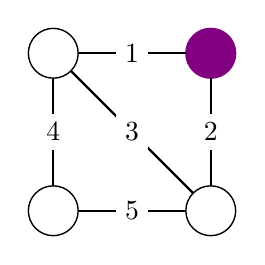
\begin{tikzpicture}[scale=0.5]
	\SetVertexNoLabel
		\Vertex[x=0 ,y=4]{A}
	\begin{scope}[VertexStyle/.append style = {color=violet}]
		\Vertex[x=4 ,y=4]{B}
	\end{scope}
		\Vertex[x=0 ,y=0]{C}
		\Vertex[x=4 ,y=0]{D}
	%	\tikzset{EdgeStyle/.append style = {bend left}}
		\Edge[label = $1$](A)(B)
		\Edge[label = $4$](A)(C)
		\Edge[label = $3$](A)(D)
		\Edge[label = $2$](B)(D)
		\Edge[label = $5$](C)(D)
	\end{tikzpicture}
\end{subfigure}
\begin{subfigure}[b]{0.25\textwidth}
	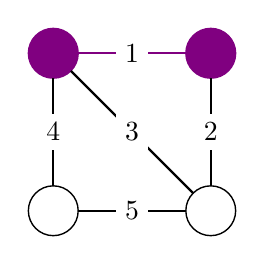
\begin{tikzpicture}[scale=0.5]
	\SetVertexNoLabel
	\begin{scope}[VertexStyle/.append style = {color=violet}]
		\Vertex[x=0 ,y=4]{A}
		\Vertex[x=4 ,y=4]{B}
	\end{scope}
		\Vertex[x=0 ,y=0]{C}
		\Vertex[x=4 ,y=0]{D}
	%	\tikzset{EdgeStyle/.append style = {bend left}}
		\Edge[label = $1$, color=violet](A)(B)
		\Edge[label = $4$](A)(C)
		\Edge[label = $3$](A)(D)
		\Edge[label = $2$](B)(D)
		\Edge[label = $5$](C)(D)
	\end{tikzpicture}
\end{subfigure}
\begin{subfigure}[b]{0.25\textwidth}
	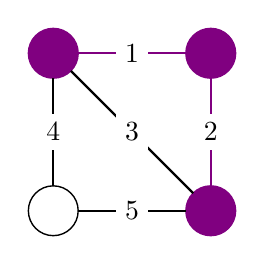
\begin{tikzpicture}[scale=0.5]
	\SetVertexNoLabel
	\begin{scope}[VertexStyle/.append style = {color=violet}]
		\Vertex[x=0 ,y=4]{A}
		\Vertex[x=4 ,y=4]{B}
	\end{scope}
		\Vertex[x=0 ,y=0]{C}
	\begin{scope}[VertexStyle/.append style = {color=violet}]
		\Vertex[x=4 ,y=0]{D}
	\end{scope}
	%	\tikzset{EdgeStyle/.append style = {bend left}}
		\Edge[label = $1$, color=violet](A)(B)
		\Edge[label = $4$](A)(C)
		\Edge[label = $3$](A)(D)
		\Edge[label = $2$, color=violet](B)(D)
		\Edge[label = $5$](C)(D)
	\end{tikzpicture}
\end{subfigure}
\begin{subfigure}[b]{0.20\textwidth}
	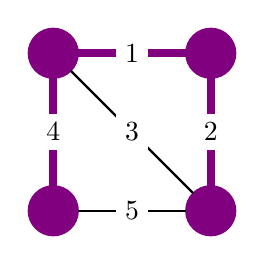
\begin{tikzpicture}[scale=0.5]
	\SetVertexNoLabel
	\begin{scope}[VertexStyle/.append style = {color=violet}]
		\Vertex[x=0 ,y=4]{A}
		\Vertex[x=4 ,y=4]{B}
		\Vertex[x=0 ,y=0]{C}
		\Vertex[x=4 ,y=0]{D}
	\end{scope}
	%	\tikzset{EdgeStyle/.append style = {bend left}}
		\Edge[label = $1$, lw=3pt, color=violet](A)(B)
		\Edge[label = $4$, lw=3pt, color=violet](A)(C)
		\Edge[label = $3$](A)(D)
		\Edge[label = $2$, lw=3pt, color=violet](B)(D)
		\Edge[label = $5$](C)(D)
	\end{tikzpicture}
\end{subfigure}
\end{figure}

Prim`s MST Algorithm pseudo-code:
\begin{itemize}
\item initialize $X=[s]$, $s \in V$ chosen arbitrarily
\item $T =\varnothing$ [invariant: X = vertices spanned by tree-so-far T]
\item while $X \neq V$:
	\begin{itemize}
		\item let $e = (u,v)$ be the cheapest edge of G with $u \in X$, $v \notin X$ 
		\item add e to T
		\item add v to X
	\end{itemize}
	i.e., increasing $\#$ of spanned vertices in cheapest way possible
\end{itemize}



\subsection{MST: Prim`s algorithm correctness proof}
\begin{theorem}Prim`s algorithm always computes an MST. [by two claims]\end{theorem}

\begin{definition} a \underline{cut} of a graph $G=(V,E)$ is a partition of V into 2 non-empty sets (there`s $2^{n-1}$ possible cuts in graph)\end{definition} 

\begin{lemma}[\textbf{empty cut lemma}] a graph is \underline{not} connected $\iff \exists$ cut $(A,B)$ with no crossing edges\end{lemma}
\begin{proof}

\textbf{[$\Leftarrow$]:} assume the RHS. Pick any $u \in A$ and $v \in B$.

Since no edges cross (A,B), there is no u-v path in G $\Rightarrow$ G not connected

\textbf{[$\Rightarrow$]:} assume the LHS. Suppose G has no u-v path.

Define A = {vertices reachable from u in G} [u`s connected components].

Define B = {all other vertices}.

Note: no edges cross the cut (A,B), otherwise A would be bigger)
\end{proof}

\begin{lemma}[\textbf{double-crossing lemma}] suppose the cycle $C \subseteq E$ has an edge crossing the cut (A,B) then so does some other edge of C (at least twice, even number in general)\end{lemma}

\begin{corollary}[\textbf{lonely cut corollary}] if e is the only edge crossing some cut (A,B), then it is not in any cycle.\end{corollary}

\begin{claim} Prim`s algorithm outputs a spanning tree\end{claim}
\begin{proof}
\begin{enumerate}
	\item algorithm maintains invariant that T spans X [by straightforward induction]
	\item can`t get stuck with $X \neq V$ (otherwise the cut (X,V-X) must be empty, by Empty-cut lemma input graph G is disconnected)
	\item no cycles ever get created in T (by lonely cut corollary - we add edge, that first crosses X and V-X - no way to create cycle)
\end{enumerate}
\end{proof}

[MST is unique if edge costs are distinct]

\begin{claim}
\textbf{Cut property}: consider an edge $e$ of $G$. Suppose there is a cut $(A,B)$ such that $e$ is the cheapest edge of $G$ that crosses it. Then $e$ belongs to the MST of $G$.
\end{claim}
\begin{proof}
Will argue by contradiction using an exchange argument [like in scheduling application]

Suppose there is an edge $e$ that is the cheapest one crossing a cut $(A,B)$, yet $e$ is not in the MST $T^*$

\underline{idea:} exchange $e$ with another edge in $T^*$ to make it even cheaper (contradiction)

\underline{note:} since $T^*$ is connected, must contain an edge $f (\neq e)$ crossing (A,B) [by cut lemma]

idea: exchange $e$ and $f$ ($f \in T^*$) to get a spanning tree cheaper than $T^*$ (contradiction) - it may work and may not work, we should exchange correct edge\dots

\underline{hope:} can always find suitable edge $e^`$ so that exchange yields bona fide spanning tree of G

let C = cycle created by adding $e$ to $T^*$

\underline{by double-crossing lemma}: some other edge $e^`$ of C [with $e^` \neq e$ and $e^` \in T^*$] crosses (A,B)

\begin{example}: $T = T^* \cup {e} - {e^`}$ is also a spanning tree\end{example}

Since $c_e < c_{e^`}$, $T$ cheaper than purported MST $T^*$	, contradictioin
\end{proof}

\begin{claim} Cut property $\Rightarrow$ Prim`s algorithm is correct\end{claim}
\begin{proof}
Prim`s algorithm outputs a spanning tree $T^*$ (by previous claim)

\underline{Key point:} Every edge $e \in T^*$ is explicitly justified by the Cut property

$\Rightarrow T^*$ is a subset of the MST

$\Rightarrow$ since $T^*$ is already a spanning tree, it must be the MST
\end{proof}



\subsection{MST: Prim`s algorithm fast implementation}
\begin{itemize}
	\item $O(n)$ iterations
	\item $O(m)$ time per iteration
	\item \textbf{$\Rightarrow O(mn)$ time}
\end{itemize}

\begin{example}use heap to store edges, with keys $=$ edge costs. This leads to $O(m \log n)$ implementation of Prim`s algorithm\end{example}

\begin{invariant}elements in heap $=$ vertices of $V-X$\end{invariant}
\begin{invariant}for $v \in V-X, key[v] =$ cheapest edge $(u,v)$ with $v \in X$ (or $+\infty$ if no such edge exist)\end{invariant}

\begin{example}can initiate heap with $O(m+n \log n) = O(m \log n)$ preprocessing ($O(m)$ to compute keys, $O(n \log n)$ for $n-1$ inserts, $m \geq n-1$ since G is connected)\\\end{example}

\underline{note}: given invariants Extract-min yields next vertex $v \notin V$ and edge $(u,v)$ crossing $(X,V-X)$ to add to X and T respectively
\\

Might need to recompute some keys to maintain Invariant2 after each Extract-min, \underline{pseudocode}:
\begin{itemize}
\item when $v$ added to $X$
\item for each edge $(v,w) \in E$
	\begin{itemize}
		\item if $w \in V-X$
		[the only vertices whose key might have dropped]
		\begin{itemize}
			\item delete $w$ from heap
			[subtle exercise - delete from heap]
			\item recompute $key[w]:= min[key[w],c_vw]$
			\item re-Insert $w$ into heap
		\end{itemize}
		[update key if needed]\\
	\end{itemize}
\end{itemize}

Heap-based implementation:
\begin{itemize}
	\item dominated by time required for heap operations
	\item $n-1$ Inserts during preprocessing
	\item $n-1$ Extract-mins (one per iteration of while loop)
	\item each edge $(v,w)$ triggers one Delete/Insert combo (when it`s first end point gets sucked into X)
	\item $\Rightarrow O(m)$ heap operations (since $m \geq n-1$ as G is connected)
	\item \textbf{$\Rightarrow O(m \log n)$ time}
\end{itemize}



\subsection{MST: Kruskal`s algorithm}
Example:
\begin{figure}[!ht]
\begin{subfigure}[b]{0.25\textwidth}
	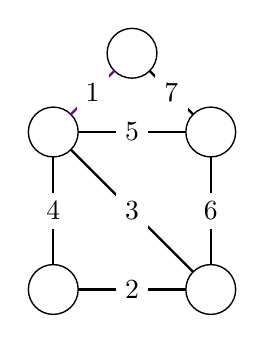
\begin{tikzpicture}[scale=0.5]
	\SetVertexNoLabel
		\Vertex[x=0 ,y=4]{A}
		\Vertex[x=4 ,y=4]{B}
		\Vertex[x=0 ,y=0]{C}
		\Vertex[x=4 ,y=0]{D}
		\Vertex[x=2 ,y=6]{E}
	%	\tikzset{EdgeStyle/.append style = {bend left}}
		\Edge[label = $5$](A)(B)
		\Edge[label = $4$](A)(C)
		\Edge[label = $3$](A)(D)
		\Edge[label = $6$](B)(D)
		\Edge[label = $2$](C)(D)
		\Edge[label = $1$, color=violet](A)(E)		
		\Edge[label = $7$](E)(B)
	\end{tikzpicture}
\end{subfigure}
\begin{subfigure}[b]{0.25\textwidth}
	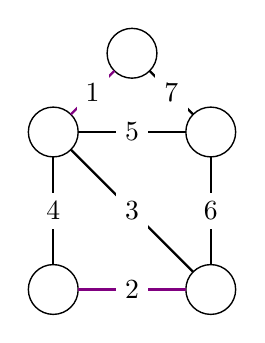
\begin{tikzpicture}[scale=0.5]
	\SetVertexNoLabel
		\Vertex[x=0 ,y=4]{A}
		\Vertex[x=4 ,y=4]{B}
		\Vertex[x=0 ,y=0]{C}
		\Vertex[x=4 ,y=0]{D}
		\Vertex[x=2 ,y=6]{E}
	%	\tikzset{EdgeStyle/.append style = {bend left}}
		\Edge[label = $5$](A)(B)
		\Edge[label = $4$](A)(C)
		\Edge[label = $3$](A)(D)
		\Edge[label = $6$](B)(D)
		\Edge[label = $2$, color=violet](C)(D)
		\Edge[label = $1$, color=violet](A)(E)		
		\Edge[label = $7$](E)(B)
	\end{tikzpicture}
\end{subfigure}
\begin{subfigure}[b]{0.25\textwidth}
	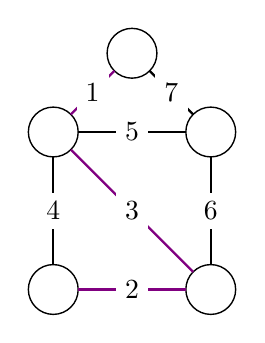
\begin{tikzpicture}[scale=0.5]
	\SetVertexNoLabel
		\Vertex[x=0 ,y=4]{A}
		\Vertex[x=4 ,y=4]{B}
		\Vertex[x=0 ,y=0]{C}
		\Vertex[x=4 ,y=0]{D}
		\Vertex[x=2 ,y=6]{E}
	%	\tikzset{EdgeStyle/.append style = {bend left}}
		\Edge[label = $5$](A)(B)
		\Edge[label = $4$](A)(C)
		\Edge[label = $3$, color=violet](A)(D)
		\Edge[label = $6$](B)(D)
		\Edge[label = $2$, color=violet](C)(D)
		\Edge[label = $1$, color=violet](A)(E)		
		\Edge[label = $7$](E)(B)
	\end{tikzpicture}
\end{subfigure}
\begin{subfigure}[b]{0.25\textwidth}
	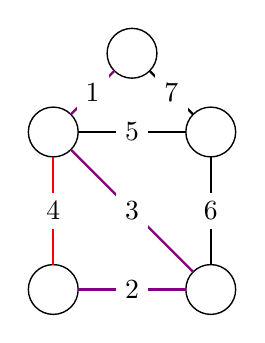
\begin{tikzpicture}[scale=0.5]
	\SetVertexNoLabel
		\Vertex[x=0 ,y=4]{A}
		\Vertex[x=4 ,y=4]{B}
		\Vertex[x=0 ,y=0]{C}
		\Vertex[x=4 ,y=0]{D}
		\Vertex[x=2 ,y=6]{E}
	%	\tikzset{EdgeStyle/.append style = {bend left}}
		\Edge[label = $5$](A)(B)
		\Edge[label = $4$, color=red](A)(C)
		\Edge[label = $3$, color=violet](A)(D)
		\Edge[label = $6$](B)(D)
		\Edge[label = $2$, color=violet](C)(D)
		\Edge[label = $1$, color=violet](A)(E)		
		\Edge[label = $7$](E)(B)
	\end{tikzpicture}
\end{subfigure}
\begin{subfigure}[b]{0.25\textwidth}
	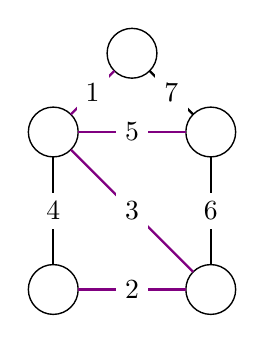
\begin{tikzpicture}[scale=0.5]
	\SetVertexNoLabel
		\Vertex[x=0 ,y=4]{A}
		\Vertex[x=4 ,y=4]{B}
		\Vertex[x=0 ,y=0]{C}
		\Vertex[x=4 ,y=0]{D}
		\Vertex[x=2 ,y=6]{E}
	%	\tikzset{EdgeStyle/.append style = {bend left}}
		\Edge[label = $5$, color=violet](A)(B)
		\Edge[label = $4$](A)(C)
		\Edge[label = $3$, color=violet](A)(D)
		\Edge[label = $6$](B)(D)
		\Edge[label = $2$, color=violet](C)(D)
		\Edge[label = $1$, color=violet](A)(E)		
		\Edge[label = $7$](E)(B)
	\end{tikzpicture}
\end{subfigure}
\begin{subfigure}[b]{0.25\textwidth}
	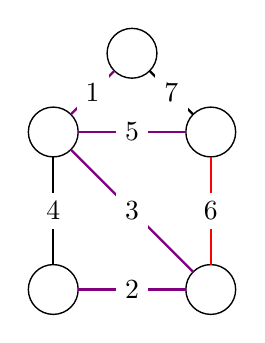
\begin{tikzpicture}[scale=0.5]
	\SetVertexNoLabel
		\Vertex[x=0 ,y=4]{A}
		\Vertex[x=4 ,y=4]{B}
		\Vertex[x=0 ,y=0]{C}
		\Vertex[x=4 ,y=0]{D}
		\Vertex[x=2 ,y=6]{E}
	%	\tikzset{EdgeStyle/.append style = {bend left}}
		\Edge[label = $5$, color=violet](A)(B)
		\Edge[label = $4$](A)(C)
		\Edge[label = $3$, color=violet](A)(D)
		\Edge[label = $6$, color=red](B)(D)
		\Edge[label = $2$, color=violet](C)(D)
		\Edge[label = $1$, color=violet](A)(E)		
		\Edge[label = $7$](E)(B)
	\end{tikzpicture}
\end{subfigure}
\begin{subfigure}[b]{0.25\textwidth}
	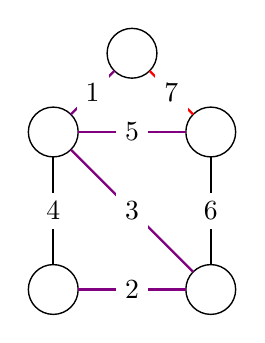
\begin{tikzpicture}[scale=0.5]
	\SetVertexNoLabel
		\Vertex[x=0 ,y=4]{A}
		\Vertex[x=4 ,y=4]{B}
		\Vertex[x=0 ,y=0]{C}
		\Vertex[x=4 ,y=0]{D}
		\Vertex[x=2 ,y=6]{E}
	%	\tikzset{EdgeStyle/.append style = {bend left}}
		\Edge[label = $5$, color=violet](A)(B)
		\Edge[label = $4$](A)(C)
		\Edge[label = $3$, color=violet](A)(D)
		\Edge[label = $6$](B)(D)
		\Edge[label = $2$, color=violet](C)(D)
		\Edge[label = $1$, color=violet](A)(E)		
		\Edge[label = $7$, color=red](E)(B)
	\end{tikzpicture}
\end{subfigure}
\end{figure}

\begin{figure}[!ht]
\begin{subfigure}[b]{\textwidth}
	\begin{center}
	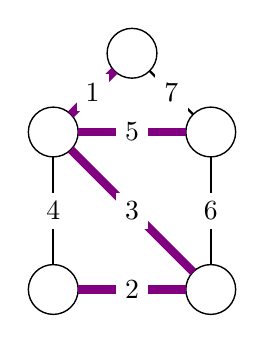
\begin{tikzpicture}[scale=0.5]
	\SetVertexNoLabel
		\Vertex[x=0 ,y=4]{A}
		\Vertex[x=4 ,y=4]{B}
		\Vertex[x=0 ,y=0]{C}
		\Vertex[x=4 ,y=0]{D}
		\Vertex[x=2 ,y=6]{E}
	%	\tikzset{EdgeStyle/.append style = {bend left}}
		\Edge[label = $5$, lw=3pt, color=violet](A)(B)
		\Edge[label = $4$](A)(C)
		\Edge[label = $3$, lw=3pt, color=violet](A)(D)
		\Edge[label = $6$](B)(D)
		\Edge[label = $2$, lw=3pt, color=violet](C)(D)
		\Edge[label = $1$, lw=3pt, color=violet](A)(E)		
		\Edge[label = $7$](E)(B)
	\end{tikzpicture}
	\end{center}
\end{subfigure}
\end{figure}

Kruskal`s MST Algorithm pseudo-code:
\begin{itemize}
\item sort edges in order of increasing cost [rename edges 1,2,3,\dots,m so that $c_1 < c_2 < \dots < c_m$]
\item $T =\varnothing$
\item for $i = 1$ to $m$
	\begin{itemize}
		\item if $T \cup [i]$ has no cycles
		\begin{itemize}
			\item add i to T
		\end{itemize}
	\end{itemize}
\item return T
\end{itemize}



\subsection{MST: Kruskal`s algorithm correctness proof}
\begin{theorem}Kruskal`s algorithm is correct\end{theorem}

\begin{proof}
Let $T^* =$ output of Kruskal`s algorithm on input graph G
\begin{enumerate}
	\item clearly $T^*$ has no cycles (by algorithm itself)
	\item $T^*$ is connected because:
	\begin{enumerate}
		\item by empty-cut lemma, only need to show that $T^*$ crosses every cut
		\item fix a cut $(A, B)$. Since $G$ connected at least one of its edges crosses $(A, B)$
		\textbf{Key point}: Kruskal`s algorithm will include first edge crossing $(A, B)$ that it sees [by lonely-cut corollary, cannot create a cycle]
	\end{enumerate}
	$\Rightarrow$ Kruskal`s algorithm outputs a spanning tree
	\item every edge of $T^*$ justified by the Cut Property (implies $T^*$ is the MST)
	\begin{enumerate}
		\item consider iteration where edge $(u, v)$ added to current set $T$ (some current state of Kruskal`s algorithm). Since $T \cup [(u, v)]$ has no cycle, T has no u-v path
		
		$\Rightarrow \exists$ empty cut $(A, B)$ separating $u$ and $v$
		
		$\Rightarrow$ by previous $2b$, no edges crossing $(A, B)$ were previously considered by Kruskal`s algorithm
		
		$\Rightarrow$ $(u, v)$ is the first (and cheapest) edge crossing $(A, B)$
		
		$\Rightarrow$ $(u, v)$ justified by the Cut Property
	\end{enumerate}
\end{enumerate}
\end{proof}



\subsection{MST: Kruskal`s algorithm via Union-Find}
Running time of straightforward implementation:
\begin{itemize}
	\item $O(m \log n)$ for sorting edges (recall $m = O(n^2)$, no parallel edges)
	\item $m$ iterations
	\item $O(n)$ to check cycles (search for other path with BFS or DFS in graph $(V, T)$, $\leq (n-1)$ edges)
	\item $\Rightarrow O(m \log n) + O(mn) = O(mn)$\\
\end{itemize}

Plan: data structure for $O(1)$-time cycle checks? $\Rightarrow O(m \log n)$
\\

Union-find data structures:
\begin{itemize}
	\item maintain partition of a set of objects
	\item $FIND(x)$: return name of a group that $x$ belongs to
	\item $UNION(c_i, c_j)$: fuse groups $c_i$ and $c_j$ into a single one.\\
\end{itemize}

For Kruskal algorithm:
\begin{itemize}
	\item objects $=$ vertices
	\item groups $=$ connected components with currently chosen edges $T$
	\item adding new edge $(u, v)$ to $T$ $\iff$ fusing connected components of $u, v$
\end{itemize}

\begin{enumerate}
	\item \textbf{Idea1}:
	\begin{itemize}
		\item maintain one linked structure per connected component of $(V, T)$
		\item each component has an arbitrary \underline{leader} vertex
		\item \textbf{Invariant}: each vertex points to the leader of its component ["name" of a component inherited from leader vertex]
		\item \textbf{Key point}: given edge $(u, v)$, can check if $u|v$ already in same component in $O(1)$ time [$\iff$ leader pointers match, $FIND(u) = FIND(v)$]
		\item $\Rightarrow O(1)$-time cycle checks!
		\item Maintaining the invariant: when new edge $(u, v)$ added to $T$, connected components of $u|v$ merge [at most $\theta(n)$ operations with pointers \underline{each time}]
	\end{itemize}
	\item \textbf{Idea2}:
	\begin{itemize}
		\item when two components merge, have smaller one inherit the leader of the larger one [maintain a size field in each component]
		\item $\theta(n)$ worst case updates to restore invariant
		\item single vertex can have $\theta(\log_2 n)$ pointers update over the courser of Kruskal`s algorithm [at each update population at least doubles]
	\end{itemize}
\end{enumerate}

Running time of fast implementation:
\begin{itemize}
	\item $O(m \log n)$ time for sorting
	\item $O(m)$ time for cycle checks [$O(1)$ per iteration]
	\item $O(n \log n)$ time overall for leader pointer updates
	\item $\Rightarrow O(m \log n)$ total running time
\end{itemize}



\subsection{MST: Application to clustering}
\textbf{Informal goal}: given $n$ "points" [web pages, images, genome fragments, etc] classify into "coherent groups"
\\

\textbf{Assumption}:
\begin{description}
	\item{(1)} as input, given a (dis)similarity measure - a distance $d(p, q)$ between each point pair
	\item{(2)} symmetric [i.e., $d(p, q) = d(q, p)$]
\end{description}

\begin{example}Euclidean distance, genome similarity, etc.\\\end{example}


\textbf{Goal}: Same cluster $\iff$ "nearby"
\\

\textbf{[Assume]:} we know k$:= \#$ of clusters desired [in practice, can experiment with a range of values]
\\

\begin{definition} call points $p|q$ \underline{separated} if they`re assigned to different clusters\end{definition}
\begin{definition} the \underline{spacing} of a $k$-clustering is $\min_{p,q-separated} d(p, q)$ [the bigger, the better]\end{definition}

\textbf{[Problem statement]:} given a distance measure d and k, compute the k-clustering with maximum spacing
\\

\textbf{Single-link clustering} pseudo-code [just like Kruskal`s MST algorithm, \underline{but stopped earlier}]:
\begin{itemize}
\item initially, each point in a separate cluster
\item repeat until only k clusters:
	\begin{itemize}
		\item let $p, q =$ closest pair of separated points (determines the current spacing)
		\item merge the clusters containing $p|q$ into a single cluster
	\end{itemize}
\end{itemize}

\begin{theorem}single-link clustering finds the $\max$-spacing $k$-clustering\end{theorem}

\begin{proof}
Let $C_1, \dots, C_k =$ greedy clustering with spacing $S$

Let $\widehat{C_1}, \dots, \widehat{C_k} =$ arbitrary other clustering

\textbf{Need to show}: spacing of $\widehat{C_1}, \dots \widehat{C_k} \leq S$

\begin{case}$\widehat{C_i}$`s are the same as the $C_i$`s [may be after renaming] $\Rightarrow$ has the same spacing S\end{case}
\begin{case}
otherwise, can find a point pair $p, q$ such that
\begin{description}
	\item{(A)} $p, q$ in the same greedy cluster $C_i$
	\item{(B)} $p, q$ in different clusters $\widehat{C_i}, \widehat{C_j}$
\end{description}

\textbf{Property of greedy algorithm}: if two points $x, y$ "directly merged" at some point, then $d(x, y) \leq S$ [distance between merged point pairs only goes up]

\begin{description}
	\item{(Easy case)} if $p, q$ directly merged at some point, $S \geq d(p, q) \geq$ spacing of $\widehat{C_1}, \dots, \widehat{C_k}$
	\item{(Tricky case)} $p, q$ "indirectly merged" through multiple direct merges.

	Let $p, a_1, \dots, a_l, q$ be the path of direct greedy merges connecting $p|a$

	\textbf{Key point}: since $p \in \widehat{C_i}$ and $q \notin \widehat{C_i}$, $\exists$ consecutive pair $a_j, a_{j+1}$ with $a_j \in \widehat{C_i}, a_{j+1} \notin \widehat{C_i}$

	$\Rightarrow S \geq d(a_j, a_{j+1})$ [since $a_j, a_{j+1}$ directly merged] $\geq$ spacing of $\widehat{C_1}, \dots, \widehat{C_k}$ [since $a_j, a_{j+1}$ separated]
\end{description}

\end{case}
\end{proof}



\subsection{Huffman codes}
\begin{definition}\underline{Binary code}: maps each character of an alphabet $\Sigma$ to a binary string\end{definition}
\begin{example}$\Sigma = a-z$ various punctuation (size $32$ overall say)\end{example}
\begin{example}\textbf{Obvious encoding} --- use the 32 5-bit binary strings to encode this $\Sigma$ (a fixed length code)\end{example}

\underline{We can do better} if some characters of $\Sigma$ are much more frequent than others, using a variable-length code.
\\

\begin{example}Suppose $\Sigma = \{A, B, C, D\}$, fixed-length encoding would be $\{00, 01, 10, 11\}$\end{example}
\begin{example}Suppose instead we use the encoding $\{0, 01, 10, 1\}$ - not enough information in encoding $001$\end{example}

\textbf{[Problem]:} with variable-length codex, not clear where one character ends and the next one begins
\\

\textbf{[Solution]:} \underline{prefix-free codes} --- make sure that for every paif $i, j \in \Sigma$, neither of the encodings $f(i), f(j)$ is a prefix of the other.
\\

\begin{example}$\{0, 10, 11, 111\}$ --- correct variable-length prefix-free encoding\end{example}
\begin{example}$A - 60~\%$, $B - 25~\%$, $C - 10~\%$, $D - 5~\%$. For fixed-length encoding -- $2$ bits/character, for variable-length encoding $\{{0, 10, 110, 111}\}$ -- $1.55$ bits/character on average\end{example}

\textbf{[Goal]:} best binary prefix-free encoding for a given set of character frequencies
\\

\textbf{[Useful fact]:} binary codes $\iff$ binary trees
\\

\begin{example}$\Sigma = \{A, B, C, D\}$
\begin{figure}[!ht]
\begin{subfigure}[b]{0.4\textwidth}
	$\{00, 01, 10, 11\}$\\
	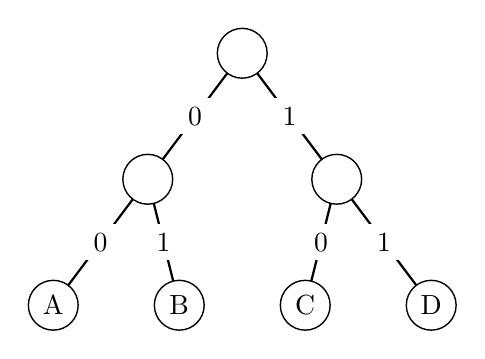
\begin{tikzpicture}[scale=0.4]
		\Vertex[x=0 ,y=0]{A}
		\Vertex[x=4 ,y=0]{B}
		\Vertex[x=8 ,y=0]{C}
		\Vertex[x=12 ,y=0]{D}
	\SetVertexNoLabel
		\Vertex[x=3 ,y=4]{E}
		\Vertex[x=9 ,y=4]{F}
		\Vertex[x=6 ,y=8]{root}
	%	\tikzset{EdgeStyle/.append style = {bend left}}
		\Edge[label = $0$](E)(A)
		\Edge[label = $1$](E)(B)
		\Edge[label = $0$](F)(C)
		\Edge[label = $1$](F)(D)
		\Edge[label = $0$](root)(E)
		\Edge[label = $1$](root)(F)
	\end{tikzpicture}
\end{subfigure}
\begin{subfigure}[b]{0.25\textwidth}
	$\{0, 01, 10, 1\}$\\
	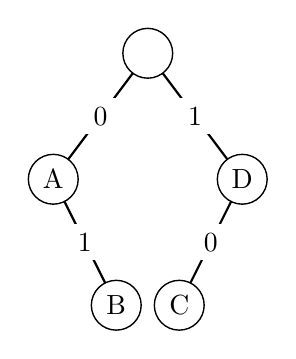
\begin{tikzpicture}[scale=0.4]
		\Vertex[x=3 ,y=4]{A}
		\Vertex[x=5 ,y=0]{B}
		\Vertex[x=7 ,y=0]{C}
		\Vertex[x=9 ,y=4]{D}
	\SetVertexNoLabel
		\Vertex[x=6 ,y=8]{root}
	%	\tikzset{EdgeStyle/.append style = {bend left}}
		\Edge[label = $1$](A)(B)
		\Edge[label = $0$](D)(C)
		\Edge[label = $0$](root)(A)
		\Edge[label = $1$](root)(D)
	\end{tikzpicture}
\end{subfigure}
\begin{subfigure}[b]{0.25\textwidth}
	$\{0, 10, 110, 111\}$ -- labels only at the leaves\\
	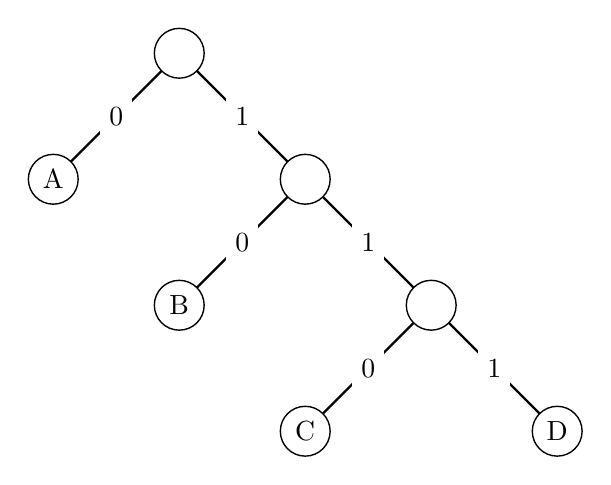
\begin{tikzpicture}[scale=0.4]
		\Vertex[x=0 ,y=8]{A}
		\Vertex[x=4 ,y=4]{B}
		\Vertex[x=8 ,y=0]{C}
		\Vertex[x=16 ,y=0]{D}
	\SetVertexNoLabel
		\Vertex[x=4 ,y=12]{root}
		\Vertex[x=8 ,y=8]{subroot1}
		\Vertex[x=12 ,y=4]{subroot2}
	%	\tikzset{EdgeStyle/.append style = {bend left}}
		\Edge[label = $0$](root)(A)
		\Edge[label = $1$](root)(subroot1)
		\Edge[label = $0$](subroot1)(B)
		\Edge[label = $1$](subroot1)(subroot2)
		\Edge[label = $0$](subroot2)(C)
		\Edge[label = $1$](subroot2)(D)
	\end{tikzpicture}
\end{subfigure}
\end{figure}

\end{example}

\textbf{[In general]:} left child edges $\iff "0"$, right child edges $\iff "1"$
\begin{itemize}
	\item for each $i \in \Sigma$, exactly one node labeled $"i"$
	\item encoding of $i \in \Sigma \iff$ bits along path from root to the node
	\item prefix-free $\iff$ labelled nodes $=$ the leaves [since prefixes $\iff$ one node an ancestor of another]
\end{itemize}

\textbf{[To decode]:} repeatedly follow path from root until you hit a leaf (unambigous since only leaves are labelled)
\\

\textbf{[Note]:} encoding length of $i \in \Sigma =$ depth of $i$ in tree
\\

\textbf{[Problem]:} input -- probability $p_i$ for each character $i \in \Sigma$. Output -- a binary tree $T$ minimizing the average encoding length $L()$

\begin{definition}if $T =$ tree with leaves $\iff$ symbols of $\Sigma$, then average encoding length $L(T) = \sum\limits_{i \in \Sigma} p_i*$[depth of i in T]\end{definition}

\textbf{Natural idea}: top down / divide and conquer (partition $\Sigma$ into two, with $50~\%$ of total frequency)

\textbf{Huffman`s (optional) idea}: build tree \underline{bottom-up} using successive mergers

\begin{observation}final encoding length of $i \in \Sigma = \#$ of mergers its subtree endures\end{observation}

\begin{figure}[ht!]
\begin{subfigure}[b]{0.5\textwidth}
	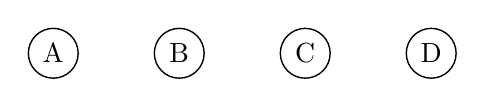
\begin{tikzpicture}[scale=0.4]
		\Vertex[x=0 ,y=0]{A}
		\Vertex[x=4 ,y=0]{B}
		\Vertex[x=8 ,y=0]{C}
		\Vertex[x=12 ,y=0]{D}
	\end{tikzpicture}
\end{subfigure}
\begin{subfigure}[b]{0.5\textwidth}
	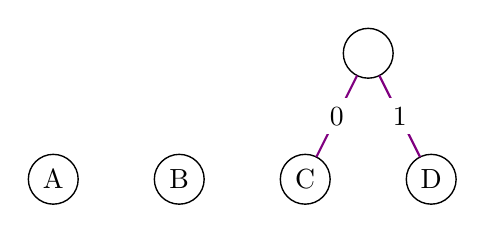
\begin{tikzpicture}[scale=0.4]
		\Vertex[x=0 ,y=0]{A}
		\Vertex[x=4 ,y=0]{B}
		\Vertex[x=8 ,y=0]{C}
		\Vertex[x=12 ,y=0]{D}
		\SetVertexNoLabel
		\Vertex[x=10 ,y=4]{subroot2}
	%	\tikzset{EdgeStyle/.append style = {bend left}}
		\Edge[label = $0$, color=violet](subroot2)(C)
		\Edge[label = $1$, color=violet](subroot2)(D)
	\end{tikzpicture}
\end{subfigure}
\begin{subfigure}[b]{0.5\textwidth}
	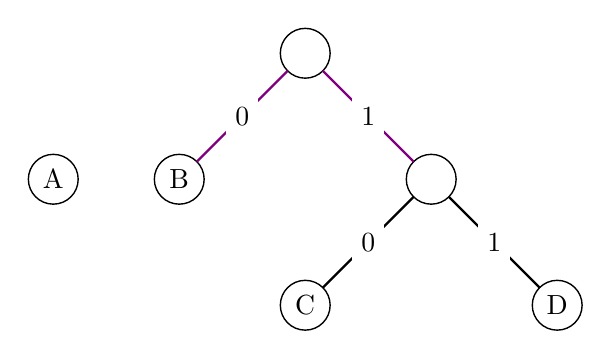
\begin{tikzpicture}[scale=0.4]
		\Vertex[x=0 ,y=4]{A}
		\Vertex[x=4 ,y=4]{B}
		\Vertex[x=8 ,y=0]{C}
		\Vertex[x=16 ,y=0]{D}
		\SetVertexNoLabel
		\Vertex[x=8 ,y=8]{subroot1}
		\Vertex[x=12 ,y=4]{subroot2}
	%	\tikzset{EdgeStyle/.append style = {bend left}}
		\Edge[label = $0$, color=violet](subroot1)(B)
		\Edge[label = $1$, color=violet](subroot1)(subroot2)
		\Edge[label = $0$](subroot2)(C)
		\Edge[label = $1$](subroot2)(D)
	\end{tikzpicture}
\end{subfigure}
\begin{subfigure}[b]{0.5\textwidth}
	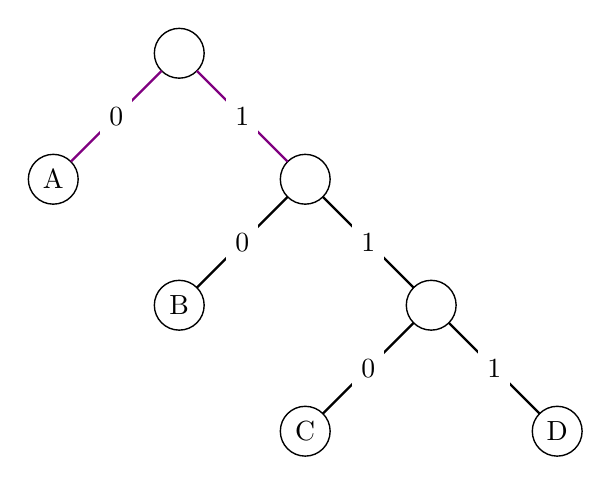
\begin{tikzpicture}[scale=0.4]
		\Vertex[x=0 ,y=8]{A}
		\Vertex[x=4 ,y=4]{B}
		\Vertex[x=8 ,y=0]{C}
		\Vertex[x=16 ,y=0]{D}
		\SetVertexNoLabel
		\Vertex[x=4 ,y=12]{root}
		\Vertex[x=8 ,y=8]{subroot1}
		\Vertex[x=12 ,y=4]{subroot2}
	%	\tikzset{EdgeStyle/.append style = {bend left}}
		\Edge[label = $0$, color=violet](root)(A)
		\Edge[label = $1$, color=violet](root)(subroot1)
		\Edge[label = $0$](subroot1)(B)
		\Edge[label = $1$](subroot1)(subroot2)
		\Edge[label = $0$](subroot2)(C)
		\Edge[label = $1$](subroot2)(D)
	\end{tikzpicture}
\end{subfigure}
\end{figure}

\textbf{Huffman`s algorithm}:
\begin{itemize}
	\item if $|\Sigma| = 2$ return (1)
	\item let $a, b \in \Sigma$ have \underline{the smallest frequences}
	\item let $\Sigma^` = \Sigma$ with $a, b$ replaced by new symbol $ab$
	\item define $p_{ab} = p_a + p_b$
	\item recursively compute $T^`$ (for the alphabet $\Sigma^`$)
	\item extend $T^`$ (with leaves $\iff \Sigma^`$) to a tree $T$ with leaves $\iff \Sigma$ by splitting leaf $ab$ into two leaves $a|b$
	\item return $T$
\end{itemize}

\begin{figure}[ht!]
\begin{subfigure}[b]{0.5\textwidth}
	(1)
	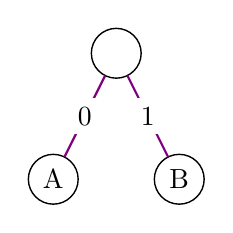
\begin{tikzpicture}[scale=0.4]
		\Vertex[x=0 ,y=0]{A}
		\Vertex[x=4 ,y=0]{B}
		\SetVertexNoLabel
		\Vertex[x=2 ,y=4]{subroot2}
	%	\tikzset{EdgeStyle/.append style = {bend left}}
		\Edge[label = $0$, color=violet](subroot2)(A)
		\Edge[label = $1$, color=violet](subroot2)(B)
	\end{tikzpicture}
\end{subfigure}
\end{figure}

\begin{theorem} [Huffman, 52] Huffman`s algorithm computes a binary tree (with leaves $\iff$ symbols of $\Sigma$) that minimizes the average encoding length\end{theorem}

\begin{proof}
By induction on $n = |\Sigma|$ (can assume $n \geq 2$)
\begin{description}
	\item{(base case)} when $n = 2$, algoruthm outputs the optimal tree (1) - 1 bit per symbol
	\item{(induction hypothesis)} algorithm solves smaller subproblem optimally (for $\Sigma^`$) - $\widehat{T^`}$
	\item{(inductive step)} fix input with $n = |\Sigma| > 2$

	Let $\Sigma^` = \Sigma$ with $a, b$ (smallest frequency) replaced by meta-symbol $ab$ ($p_{ab} = p_a + p_b$)

	Exact correspondence $T \iff T^`$. Let trees for $\Sigma$ that have $a, b$ as siblings ($T1$) - $X_{ab}$

	\textbf{important}: for every such pair $T^`$ and $T$, $L(T)-L(T^`) = p_a(d+1) + p_b(d+1) - (p_a+p_b)d = p_a + p_b$ - \textbf{independent of $T, T^`$}

	\textbf{upshot}: corresponding tree $\widehat{T^`}$ minimizes $L(T)$ for $\Sigma$ over all trees in $X_{ab}$ (where $a|b$ are siblings)

	\textbf{key lemma} complete`s proof of theorem
\end{description}
\end{proof}

\begin{lemma}there is an optimal tree (for $\Sigma$) in $X_{ab}$ [i.e. $a, b$ were "safe" to merge]\end{lemma}

\begin{proof}
\textbf{Intuition}: can make an optimal tree better by pushing $a|b$ as deep as possible (since $a, b$ have smallest frequencies)

[By exchange argument]
\\

Let $T^*$ be any tree that minimizes $L(T)$ for $\Sigma$

Let $x, y$ be siblings at the deepest level of $T^*$

\textbf{exchange}: obtain $\widehat{T}$ from $T^*$ by swapping labels $a \leftarrow\rightarrow x, b \leftarrow\rightarrow y$
\\

[note]: $\widehat{T} \in X_{ab}$ by choice of $x, y$
\\

$L(T^*) - L(\widehat{T}) = (p_x-p_a)[$depth of $x$ in $T^* -$ depth of $a$ in $T^*] + (p_y-p_b)[$depth of $y$ in $T^* -$ depth of b in $T^*] \geq 0$, since

$(p_x-p_a), (p_y-p_b) \geq 0$ (smallest frequency of $a,b$) and by choice of $x, y$

$\Rightarrow L(\widehat{T}) \leq L(T^*)$

$\Rightarrow \widehat{T}$ also optimal
\end{proof}

\textbf{Running time}:
\begin{itemize}
	\item \underline{naive implementation} - $O(n^2)$, where $n = |\Sigma|$
	\item \underline{speed ups} use a heap (repeated minimum computations)

	keys - frequences

	after extracting the two smallest-frequency symbols, re-Insert the new meta-symbol [key - sum of the $2$ old one`s]

	$\Rightarrow$ iterative, $O(n \log n)$ implementation
	\item \underline{even faster} sorting + $O(n)$ additional work

	\begin{example}manage (meta-)symbols using two queues\end{example}
\end{itemize}
\end{document}